\documentclass{article}
\usepackage{amsmath}
\usepackage{amssymb}
\usepackage{graphicx}
\usepackage{hyperref}
\usepackage[version=4]{mhchem}


\begin{document}
\(A B C D\) is a parallelogram. \(A\) circle is drawn such that it passes through \(A, B, C\) and meets the side \(D A\) at \(E\). Find \(D E\) if \(A B=4\), and \(B E=5\).

Solution: \(\frac{16}{5}\).\\
Method 1:\\
\centering

\includegraphics[width=\textwidth]{images/167.jpg}

Connect \(A C, C E\).\\
Since \(A B C D\) is a parallelogram, \(B C=D A, A B=D C=4 . \angle A C D=\angle C B A=\alpha\) (alternate interior angles)\\
\(\angle A B C=\angle A C D=\alpha\) (they face the same \(\operatorname{arc} A C\) ).\\
Thus \(A C=B C\).\\
Since \(A E / / B C, A E C B\) is an isosceles trapezoid. So \(B E=\) \(A C=5\).\\
Since \(A D=B C=A C=5\).\\
\centering
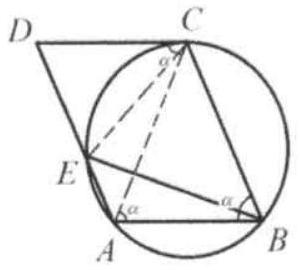
\includegraphics[width=\textwidth]{images/167(2).jpg}

Therefore, \(D C^{2}=D A \times D E \Rightarrow 4^{2}=5 \times D E \Rightarrow D E=\frac{4^{2}}{5}=\frac{16}{5}\).

Method 2:\\
Connect \(A C, C E\).\\
Since \(A B C D\) is a parallelogram, \(A B=D C=4 . \angle D=\angle C B A=\beta\) (alternate interior angles).\\
Since \(A E / / B C, A E C B\) is an isosceles trapezoid. So \(A B=C E=4\), and \(B E=A C=\) 5.\\
\(\angle D C E=\angle A C D=\alpha\) (they face the arcs of the same length arcs \(C E, A B)\).\\
Then triangles \(C D E\) and \(C B A\) are similar to each other, so the following equality holds true: \(\frac{C E}{D E}=\frac{A C}{A B}\)\\
\centering

\includegraphics[width=\textwidth]{images/168.jpg}\\
\(\Rightarrow \quad \frac{4}{D E}=\frac{5}{4}\)\\
\(\Rightarrow \quad D E=\frac{4^{2}}{5}=\frac{16}{5}\).
\end{document}
